\begin{figure}
    \centering
    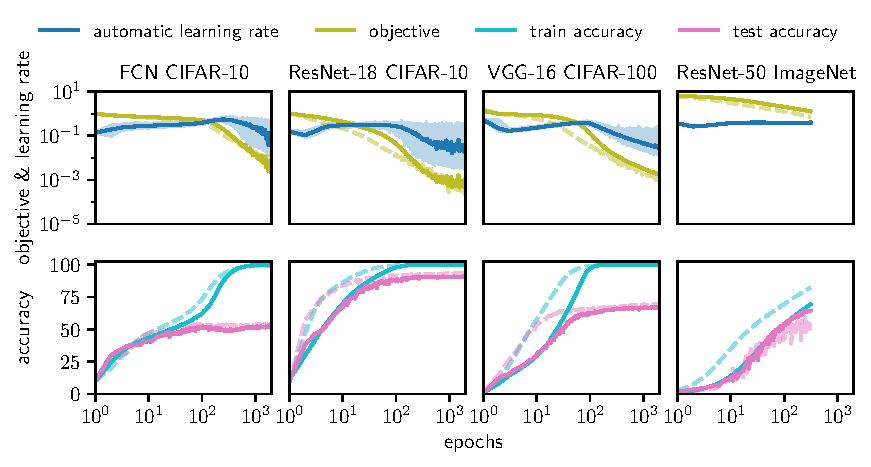
\includegraphics[width=\textwidth]{figures/pdf/plot1_full}
    \caption{\captiontitle{Benchmarking automatic gradient descent on a range of architectures and datasets.} Solid lines are AGD and faint dashed lines are tuned Adam except for ImageNet where the dashed line is SGD with a fixed learning rate of 0.1. ImageNet used cross-entropy loss with a mini-batch size of 1024. The other experiments used square loss with a mini-batch size of 128.
    The \captiontitle{top row} plots the automatic learning rate ($\eta$ in the main text) and objective value. The maximum and minimum learning rate for each epoch is included in addition to the mean for the first three plots. The \captiontitle{bottom row} shows the train and test accuracy.
    }\label{fig:1}
\end{figure}